\section{Runtime Scaling with Model Input Count}
\label{sec:scaling}
\subsection{Recorded Inputs and Replay Workloads}
The runtime-only experiment fixes the checkpoint and a 30-frame cohort while
varying $n$ from one to twenty~\cite{recordruntime}. Every frame provides five
recorded vehicle inputs. For $n\leq5$, ego 1 is kept and the nearest recorded
vehicles are added. For $n>5$, the same five scans and their recorded pairwise
poses are cycled into additional tensors and active slots. For example,
$n=20$ contains four copies of the five recorded inputs.

Consequently, $n$ denotes model input slots. Above five, this experiment tests
computational load rather than perception from newly observed vehicles. No
AP or box postprocessing is computed in this runtime-only sweep. Its role is
to expose execution cost under increasing workload, not to predict detection
gains with twenty independent vehicles.

\begin{table}[htbp]
\centering
\caption{Input reuse and original fine-pair workload at selected slot counts.}
\label{tab:replay-workload}
\begin{ReportTable}{rrrL}
\ReportTableHead
\ReportTH{Slots $n$} & \ReportTH{Distinct recorded inputs} & \ReportTH{Ordered pairs $n^2$} & \ReportTH{Input composition} \\
1 & 1 & 1 & Ego input \\
5 & 5 & 25 & Five recorded inputs \\
10 & 5 & 100 & Two cycles of the five inputs \\
20 & 5 & 400 & Four cycles of the five inputs \\
\end{ReportTable}
\end{table}

Table~\ref{tab:replay-workload} makes the workload increase explicit. The
implementation allocates additional tensors and active slots even when
the underlying scan is repeated. Encoding, pairwise collaboration, and
decoding therefore process a larger group. Cycling recorded poses keeps
each replay tied to its source observation, rather than placing a newly
observed vehicle at an invented location.

\subsection{Timing Boundary}
Each condition uses the same 30 frames in three trials, with twenty warmup
forwards per condition and trial. Condition order is shuffled with seed zero.
This gives 90 timed samples per $n$, or 1,800 timed forwards and 1,200 warmup
forwards across the sweep. Inputs are already on the GPU, and CUDA is
synchronized before and after each measured forward.

The forward timer includes the encoder, pairwise fusion, decoder, and
detection heads for the \emph{entire $n$-slot group}. It excludes file reads,
CPU packing, raw LiDAR preprocessing, input transfer, model loading, warmups,
and output checks. These times are not per-vehicle wireless latency and are
not the duration of the whole data-loading/evaluation pipeline.

\subsection{Results}
Median full-group forward time increases from \ReportRuntimeStart\ ms at
$n=1$ to \ReportRuntimeEnd\ ms at $n=20$, a factor of
\ReportRuntimeFactor. Table~\ref{tab:runtime} reports every condition, with
the 95th percentile (P95) of its 90 timing samples. P95 describes the observed
tail of those timings; it is not a confidence interval for the median.

\begin{table}[htbp]
\centering
\caption{Runtime-only sweep on the fixed 30-frame cohort. The rule after
$n=5$ marks the change from distinct recorded inputs to replayed-input
workloads. Timings refer to full-group forward execution.}
\label{tab:runtime}
\input{runtime-table.generated}
\end{table}

\begin{figure}[htbp]
\centering
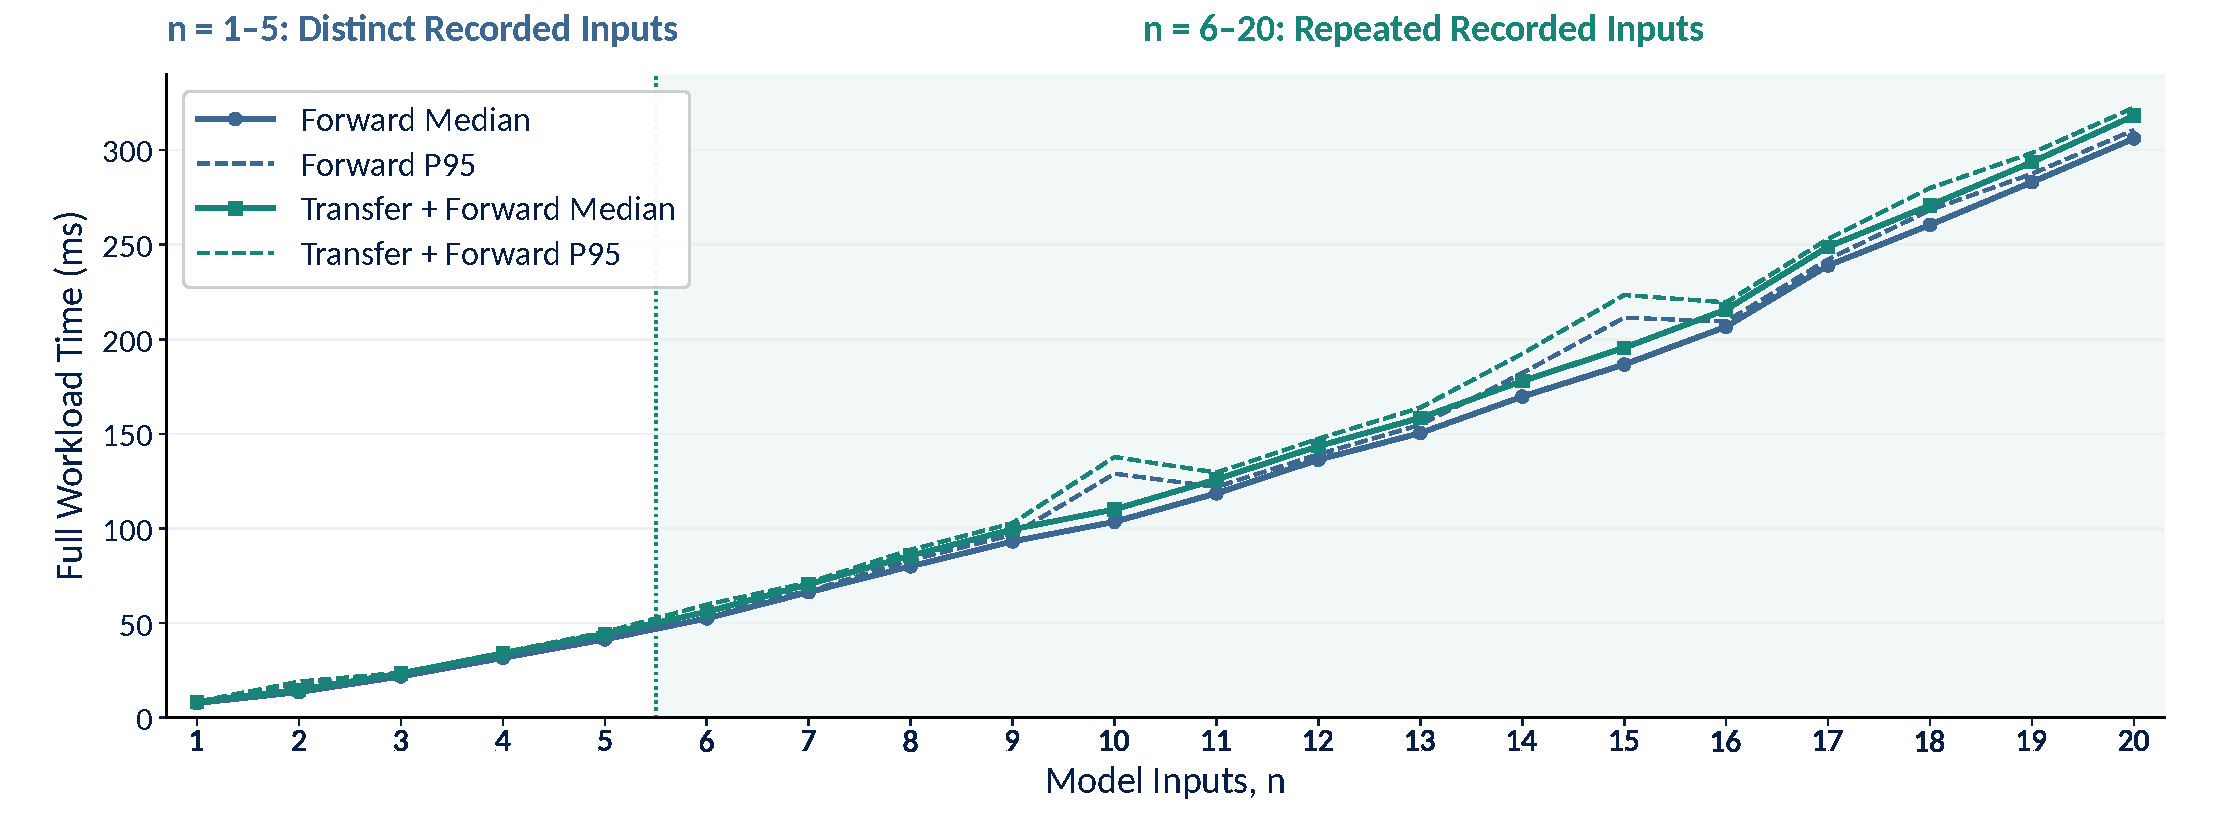
\includegraphics[width=\linewidth]{experiments/w45-2026-11-04/runtime-scaling-v1.pdf}
\caption[Recorded runtime scaling from one to twenty slots]{Saved
runtime-scaling figure. Forward timings and transfer-plus-forward
timings have different boundaries; only the former are tabulated in
Table~\ref{tab:runtime}. The plot retains the original measured medians and
P95 values~\cite{recordruntime}.}
\label{fig:runtime}
\end{figure}

The growth is consistent with the increasing cost of a pipeline containing
all-pair feature collaboration. At $n=20$, the original graph evaluates
400 ordered fine-resolution pairs including self pairs, compared with one
at $n=1$. The measured runtime ratio is not required to equal the pair-count
ratio because other stages, batching, and hardware behavior also contribute.
The experiment does not fit a universal complexity law or isolate fusion
time from the rest of the model.

The two timing boundaries in Figure~\ref{fig:runtime} are part of the
experiment setup. The forward-only series matches the tabulated GPU-ready
workload. The transfer-plus-forward series includes an additional input
transfer stage. Neither includes all operations of the full-test evaluation,
such as file access, prediction export, and AP calculation. Separating
these boundaries avoids attributing the whole evaluation duration to the
network's forward pass.
